% The SHA-2 message schedule [FIPS 180-4, §6.2.2 step 1, §6.4.2 step 1]:
%   W_t = M_t for t < 16,  W_t = σ1(W_{t-2}) + W_{t-7} + σ0(W_{t-15}) + W_{t-16} otherwise.
% Original drawing for the Hash library.
\documentclass[tikz,border=6pt]{standalone}
\usepackage[T1]{fontenc}
\usepackage{lmodern}
% Shared style for the Hash diagrams.
% Palette: Okabe–Ito (colour-blind safe). Every diagram is drawn on an opaque white card so it
% stays legible on dark page themes.
\usetikzlibrary{arrows.meta,positioning,calc,fit,backgrounds}
\definecolor{hsblue}{HTML}{0072B2}
\definecolor{hsorange}{HTML}{E69F00}
\definecolor{hsgreen}{HTML}{009E73}
\definecolor{hsvermilion}{HTML}{D55E00}
\definecolor{hspurple}{HTML}{CC79A7}
\definecolor{hsink}{HTML}{1F2933}
\tikzset{
  >={Stealth[length=2.2mm]},
  every node/.style={font=\sffamily\small, text=hsink},
  wire/.style={draw=hsink, line width=0.6pt, ->},
  reg/.style={draw=hsink, line width=0.6pt, fill=hsblue!12, minimum width=9mm, minimum height=7mm},
  fn/.style={draw=hsink, line width=0.6pt, fill=hsorange!25, rounded corners=2pt, minimum width=10mm, minimum height=6mm},
  input/.style={draw=hsink, line width=0.6pt, fill=hsgreen!20, minimum width=9mm, minimum height=6mm},
  add/.style={circle, draw=hsink, line width=0.6pt, fill=white, inner sep=0pt, minimum size=5mm, font=\sffamily\bfseries},
  card/.style={fill=white, rounded corners=4pt},
}

\begin{document}
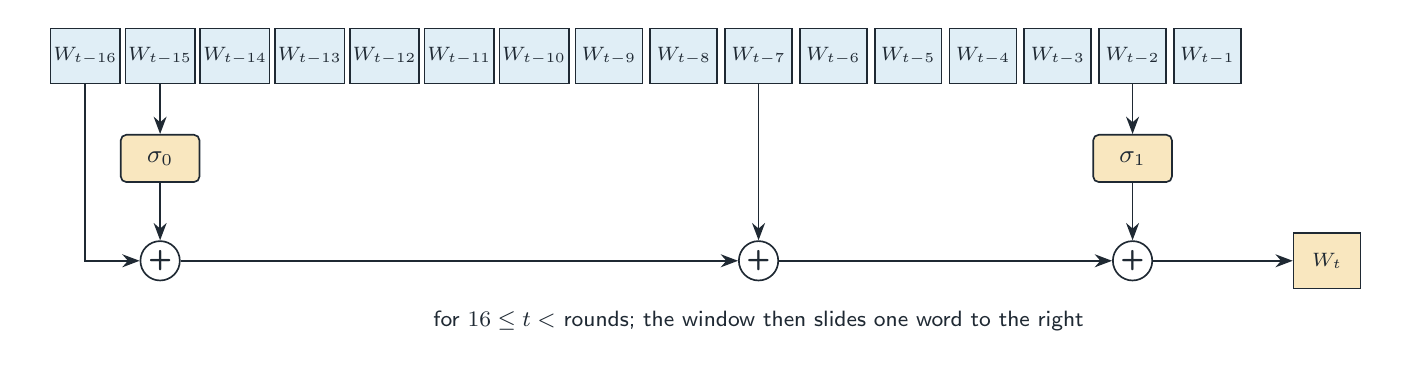
\begin{tikzpicture}
  \def\dx{0.95}
  % A window of the sixteen most recent words.
  \foreach \lbl [count=\i from 0] in {16,15,14,13,12,11,10,9,8,7,6,5,4,3,2,1} {
    \node[reg, minimum width=8.5mm, inner sep=1pt] (w\lbl) at (\i*\dx, 0) {\scriptsize $W_{t-\lbl}$};
  }
  \node[reg, minimum width=8.5mm, inner sep=1pt, fill=hsorange!25] (wt) at (16.6*\dx, -2.6) {\scriptsize $W_t$};
  \node[fn] (s0) at (w15 |- 0,-1.3) {$\sigma_0$};
  \node[fn] (s1) at (w2 |- 0,-1.3) {$\sigma_1$};
  \node[add] (p1) at (w7 |- 0,-2.6) {+};
  \node[add] (p2) at (w15 |- 0,-2.6) {+};
  \node[add] (p3) at (w2 |- 0,-2.6) {+};
  \draw[wire] (w16.south) |- (p2.west);
  \draw[wire] (w15.south) -- (s0.north);
  \draw[wire] (s0.south) -- (p2.north);
  \draw[wire] (p2.east) -- (p1.west);
  \draw[wire] (w7.south) -- (p1.north);
  \draw[wire] (p1.east) -- (p3.west);
  \draw[wire] (w2.south) -- (s1.north);
  \draw[wire] (s1.south) -- (p3.north);
  \draw[wire] (p3.east) -- (wt.west);
  \node[font=\sffamily\footnotesize, anchor=north] at ($(p1.south)+(0,-0.25)$)
    {for $16 \le t <$ rounds; the window then slides one word to the right};
  \begin{scope}[on background layer]
    \node[card, fit=(w16)(w1)(wt), inner sep=8pt, minimum height=4.2cm, yshift=-5mm] {};
  \end{scope}
\end{tikzpicture}
\end{document}
